\begin{Figure}

    \SECTION{2.2 Modelling Olfactory Bulb}
    \centering
    \begin{tikzpicture}
        \node[] (aditya) {
            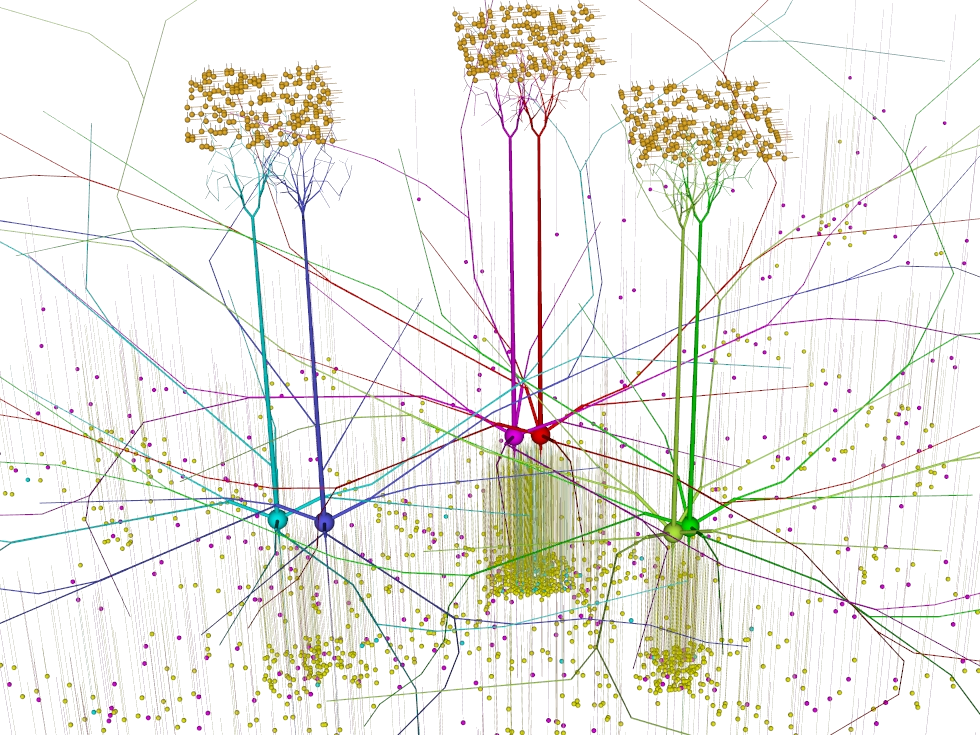
\includegraphics[width=\textwidth]{./images/fullmodel_moogli.png}
        };
    \end{tikzpicture}
    \vspace{1cm}

    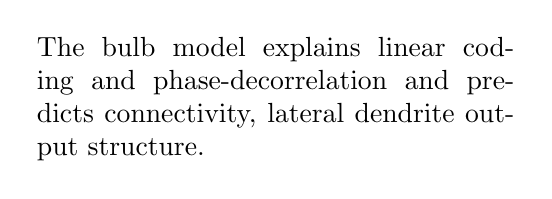
\begin{tikzpicture}
        \node[] (caption) {
            \begin{minipage}{0.5\textwidth}
                \TEXT{
                     The bulb model explains linear coding and phase-decorrelation and
                    predicts connectivity, lateral dendrite output structure.} 
            \end{minipage}
        };
    \end{tikzpicture} \hfill%
    \begin{tikzpicture}
        \node[] (result) {
            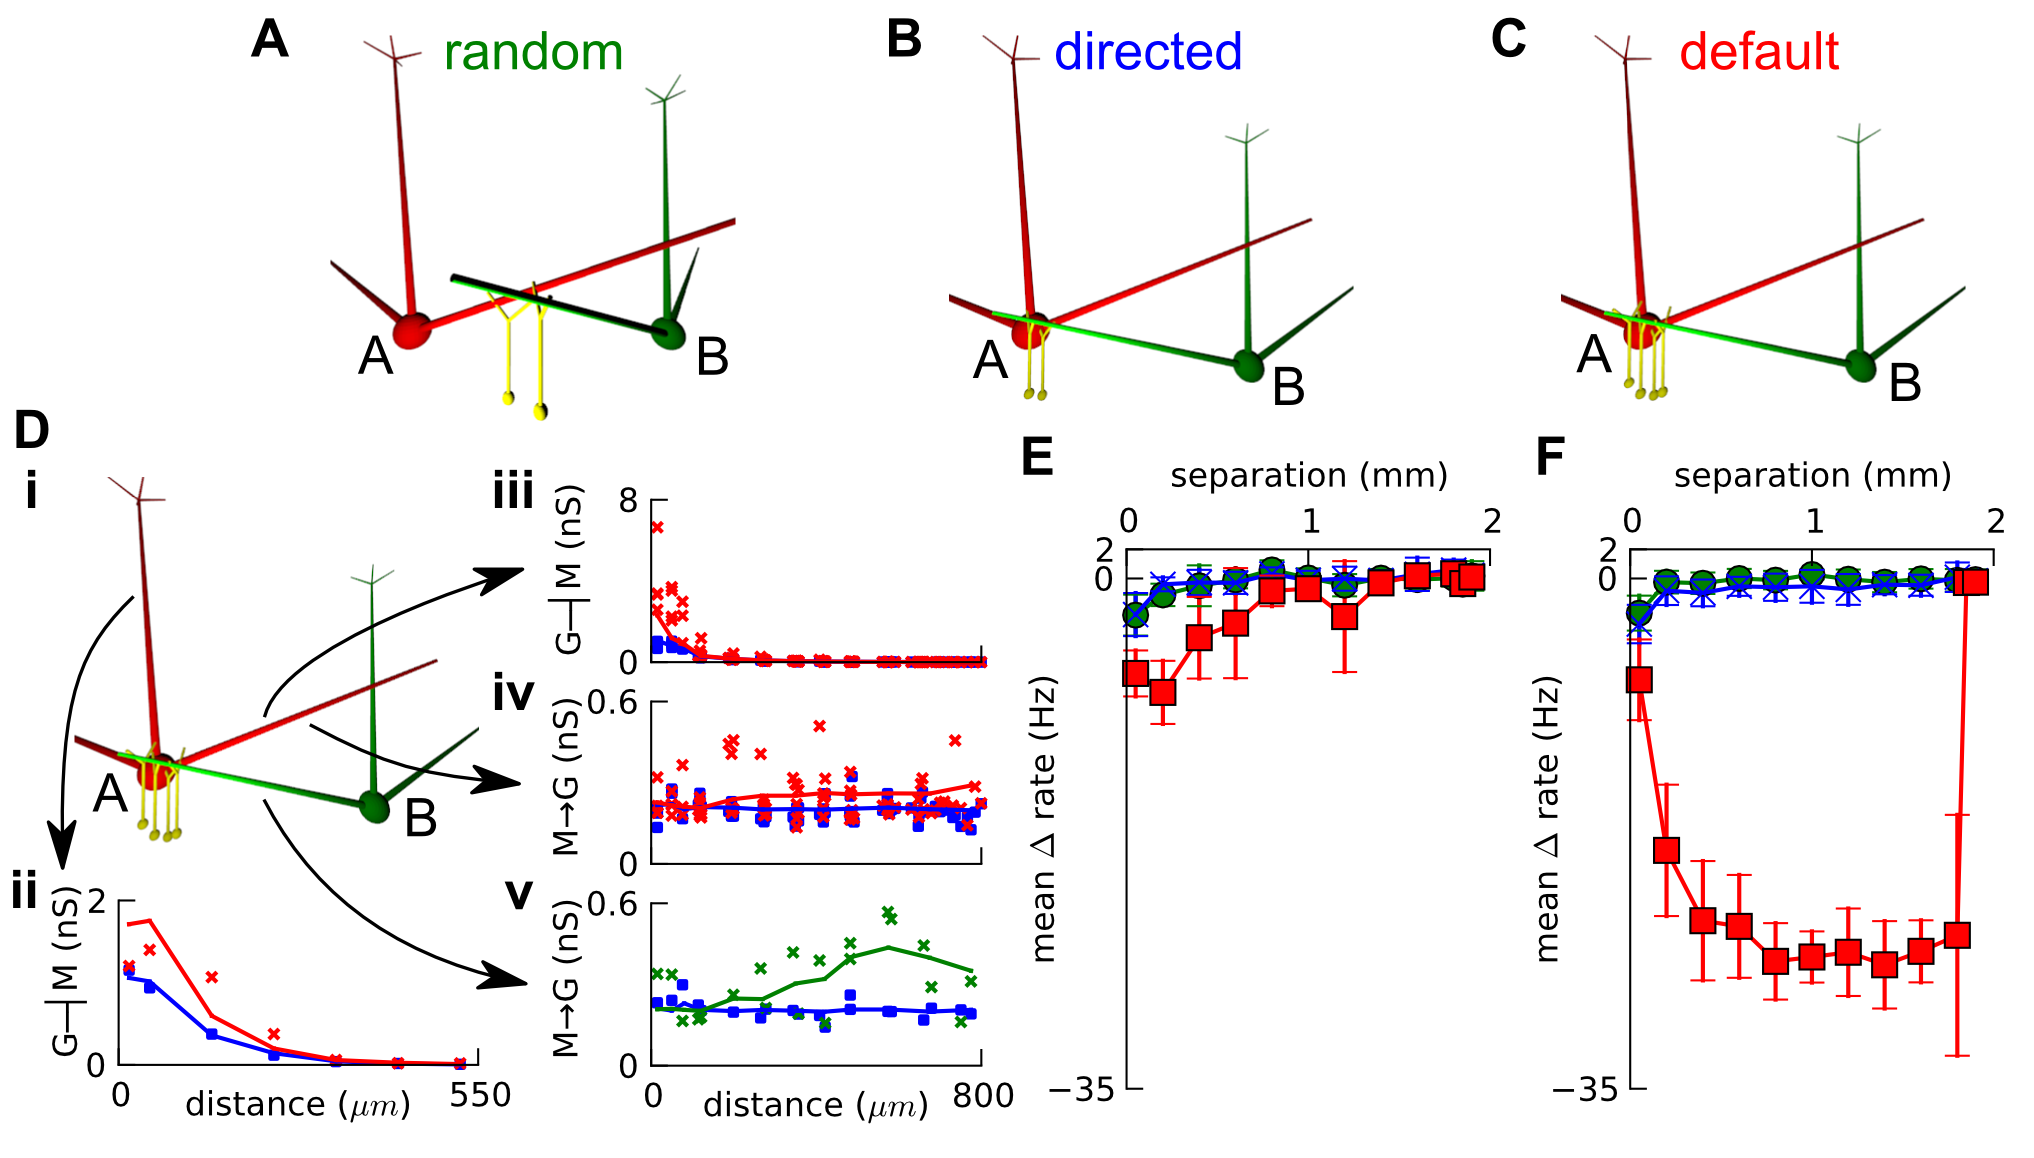
\includegraphics[width=0.45\textwidth]{./images/aditya_work.png}
        };
    \end{tikzpicture}

    %% One more model here.
    \raggedright
    \SECTION{2.3 Modelling Cortex}

    \TEXT{\bf Predicts:}

    \centering
    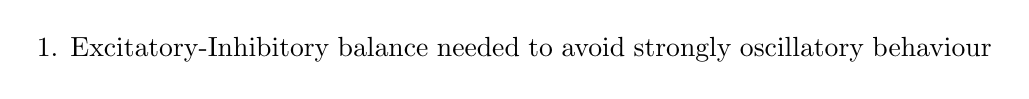
\begin{tikzpicture}
        \node [] (label) {
            \begin{minipage}{\textwidth}
                \TEXT{1. Excitatory-Inhibitory balance needed to avoid strongly oscillatory
                    behaviour}
            \end{minipage}
        };
    \end{tikzpicture}
    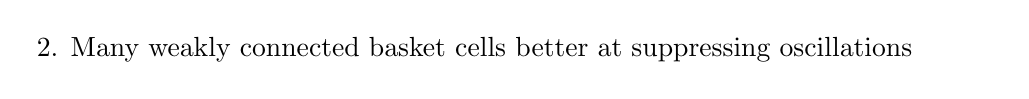
\begin{tikzpicture}
        \node [] (label) {
            \begin{minipage}{\textwidth}
                \TEXT{2. Many weakly connected basket cells better at suppressing
                    oscillations}
            \end{minipage}
        };
    \end{tikzpicture}

    \vspace{-1cm}
    \begin{tikzpicture}
        \node[] (robust) {
            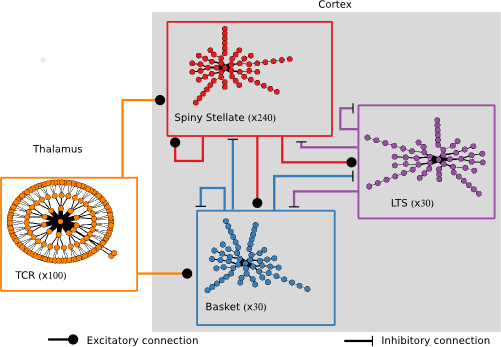
\includegraphics[width=0.9\textwidth]{./images/subha.png}
        };
    \end{tikzpicture}

\end{Figure}


